\documentclass{standalone}
\usepackage{tikz}
\usetikzlibrary{patterns, positioning}
\usepackage[sfdefault]{ClearSans} %% option 'sfdefault' activates Clear Sans as the default text font
\usepackage[T1]{fontenc}

\begin{document}
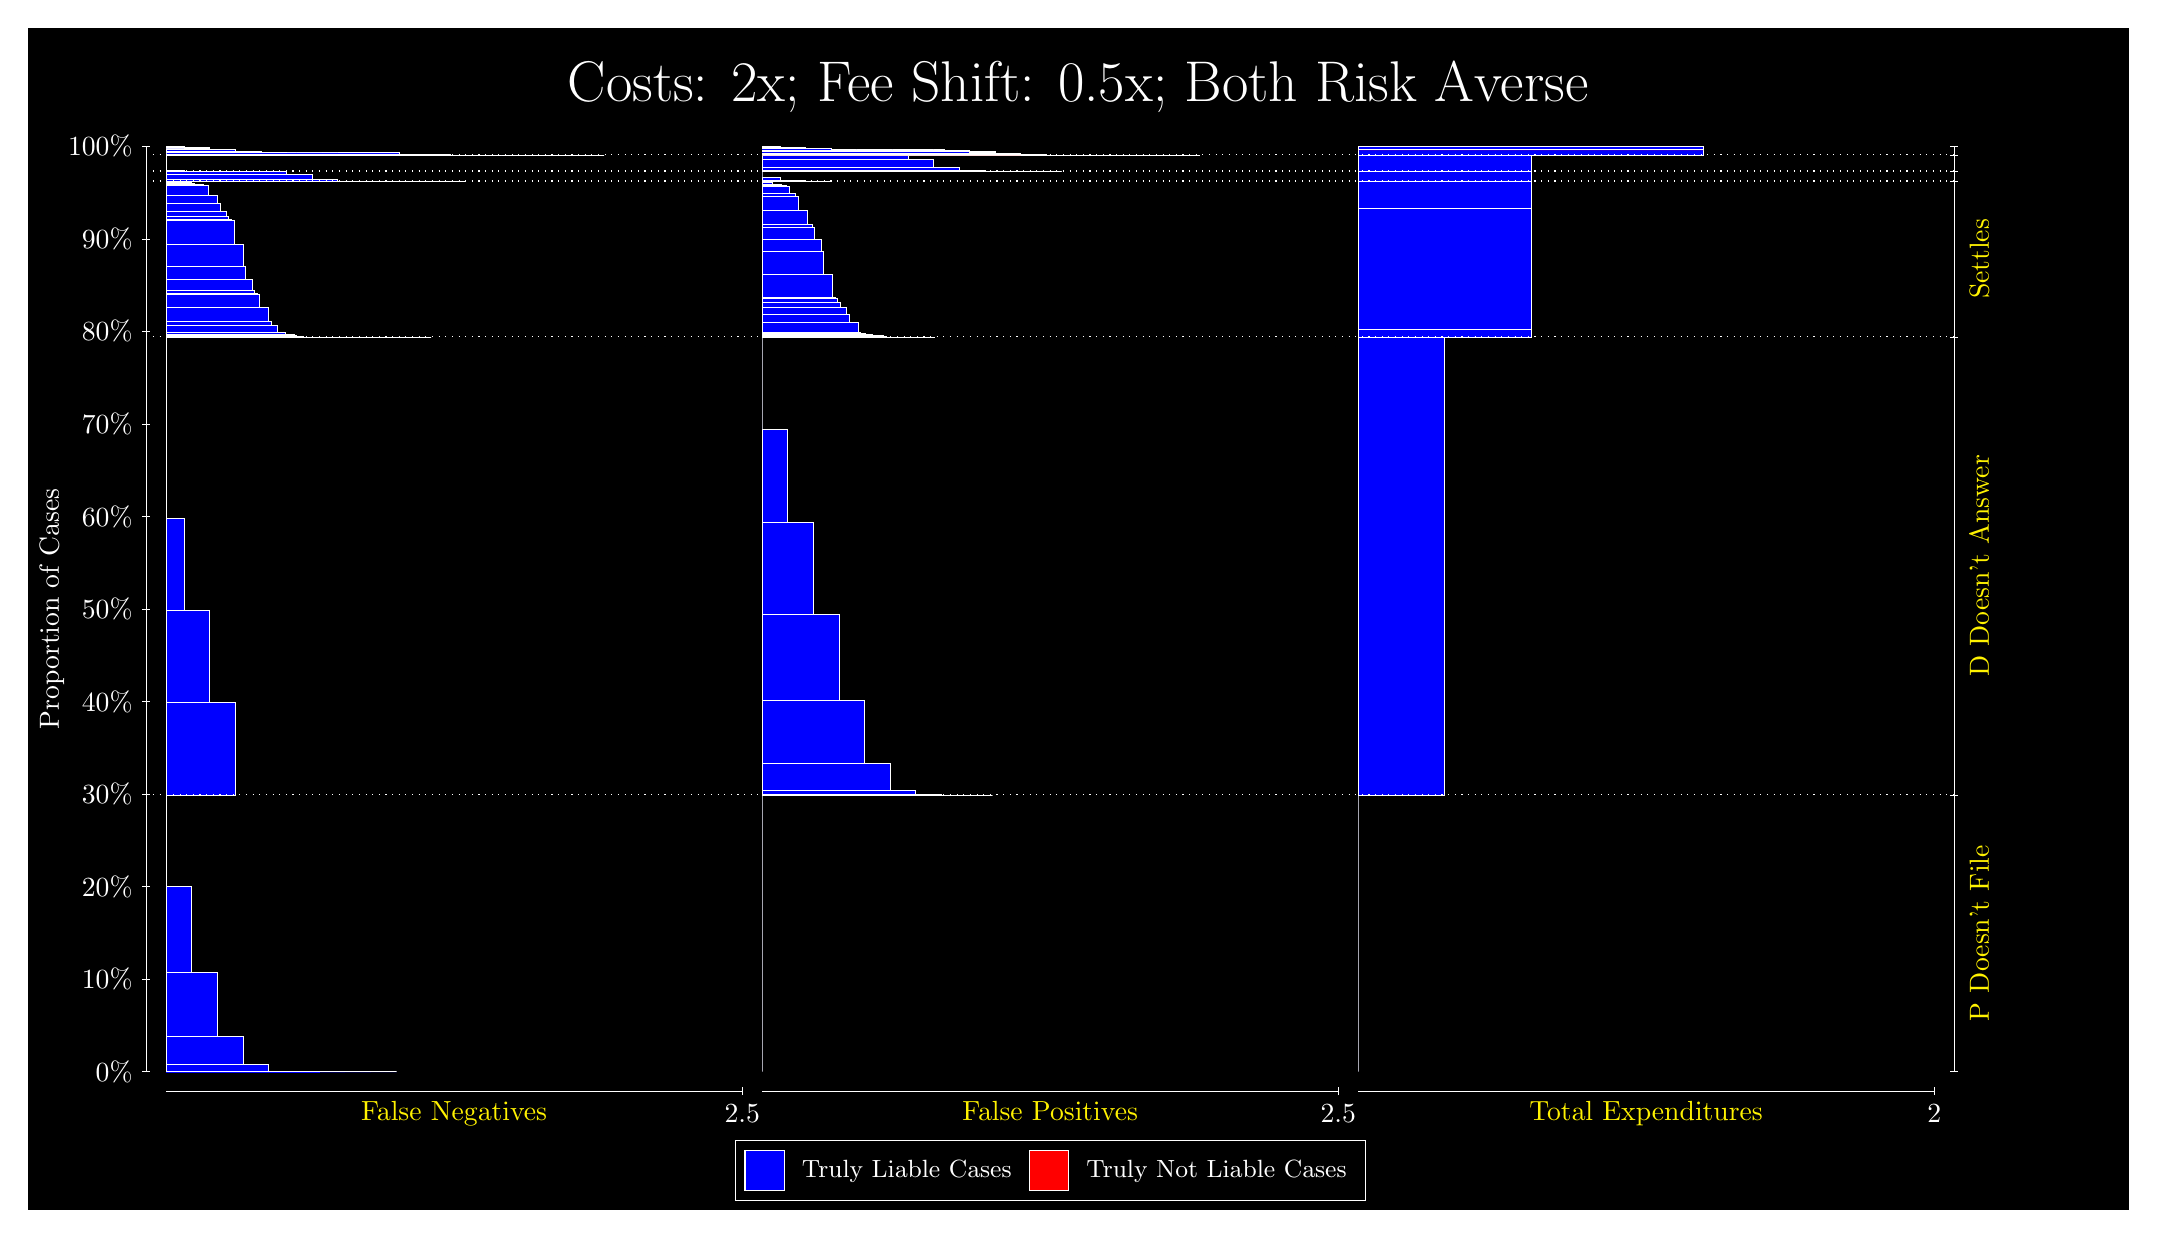
\begin{tikzpicture}
\draw[fill=black] (0,0) rectangle (26.667,15);
\draw[text=white] (0,13.5) rectangle (26.667,15) node[midway] {\huge Costs: 2x; Fee Shift: 0.5x; Both Risk Averse};
\draw[white, very thin] (1.5,1.75) -- (1.5,13.5);
\node[rotate=90, text=white, anchor=center] at (0.3, 7.625) {Proportion of Cases};
\draw[white, very thin] (1.45,1.75) -- (1.55,1.75);
\node[text=white, anchor=east] at (1.45, 1.75) {0\%};
\draw[white, very thin] (1.45,2.925) -- (1.55,2.925);
\node[text=white, anchor=east] at (1.45, 2.925) {10\%};
\draw[white, very thin] (1.45,4.1) -- (1.55,4.1);
\node[text=white, anchor=east] at (1.45, 4.1) {20\%};
\draw[white, very thin] (1.45,5.275) -- (1.55,5.275);
\node[text=white, anchor=east] at (1.45, 5.275) {30\%};
\draw[white, very thin] (1.45,6.45) -- (1.55,6.45);
\node[text=white, anchor=east] at (1.45, 6.45) {40\%};
\draw[white, very thin] (1.45,7.625) -- (1.55,7.625);
\node[text=white, anchor=east] at (1.45, 7.625) {50\%};
\draw[white, very thin] (1.45,8.8) -- (1.55,8.8);
\node[text=white, anchor=east] at (1.45, 8.8) {60\%};
\draw[white, very thin] (1.45,9.975) -- (1.55,9.975);
\node[text=white, anchor=east] at (1.45, 9.975) {70\%};
\draw[white, very thin] (1.45,11.15) -- (1.55,11.15);
\node[text=white, anchor=east] at (1.45, 11.15) {80\%};
\draw[white, very thin] (1.45,12.325) -- (1.55,12.325);
\node[text=white, anchor=east] at (1.45, 12.325) {90\%};
\draw[white, very thin] (1.45,13.5) -- (1.55,13.5);
\node[text=white, anchor=east] at (1.45, 13.5) {100\%};

\draw[white, very thin] (24.457,1.75) -- (24.457,13.5);
\draw[white, very thin] (24.407,1.75) -- (24.507,1.75);
\node[anchor=west] at (24.407, 1.75) {};
\draw[white, very thin] (24.407,5.264) -- (24.507,5.264);
\node[anchor=west] at (24.407, 5.264) {};
\draw[white, very thin] (24.407,11.08) -- (24.507,11.08);
\node[anchor=west] at (24.407, 11.08) {};
\draw[white, very thin] (24.407,13.059) -- (24.507,13.059);
\node[anchor=west] at (24.407, 13.059) {};
\draw[white, very thin] (24.407,13.186) -- (24.507,13.186);
\node[anchor=west] at (24.407, 13.186) {};
\draw[white, very thin] (24.407,13.391) -- (24.507,13.391);
\node[anchor=west] at (24.407, 13.391) {};
\draw[white, very thin] (24.407,13.5) -- (24.507,13.5);
\node[anchor=west] at (24.407, 13.5) {};

\draw[white, very thin, fill=blue] (1.75,1.75) rectangle (4.6775,1.75);
\draw[white, very thin, fill=blue] (1.75,1.75) rectangle (4.3523,1.75);
\draw[white, very thin, fill=blue] (1.75,1.75) rectangle (4.027,1.75);
\draw[white, very thin, fill=blue] (1.75,1.75) rectangle (3.7017,1.7503);
\draw[white, very thin, fill=blue] (1.75,1.7503) rectangle (3.3764,1.7576);
\draw[white, very thin, fill=blue] (1.75,1.7576) rectangle (3.0511,1.8361);
\draw[white, very thin, fill=blue] (1.75,1.8361) rectangle (2.7258,2.1984);
\draw[white, very thin, fill=blue] (1.75,2.1984) rectangle (2.4006,3.0086);
\draw[white, very thin, fill=blue] (1.75,3.0086) rectangle (2.0753,4.0995);
\draw[white, very thin, fill=red] (1.75,4.0995) rectangle (1.75,4.0995);
\draw[white, very thin, fill=blue] (1.75,4.0995) rectangle (1.75,5.264);
\draw[white, very thin, fill=blue] (1.75,5.264) rectangle (2.6283,6.439);
\draw[white, very thin, fill=blue] (1.75,6.439) rectangle (2.303,7.6137);
\draw[white, very thin, fill=blue] (1.75,7.6137) rectangle (1.9777,8.7813);
\draw[white, very thin, fill=red] (1.75,8.7813) rectangle (1.75,8.7813);
\draw[white, very thin, fill=blue] (1.75,8.7813) rectangle (1.75,11.08);
\draw[white, very thin, fill=blue] (1.75,11.08) rectangle (5.1167,11.08);
\draw[white, very thin, fill=blue] (1.75,11.08) rectangle (4.8239,11.08);
\draw[white, very thin, fill=blue] (1.75,11.08) rectangle (4.7914,11.08);
\draw[white, very thin, fill=blue] (1.75,11.08) rectangle (4.6775,11.08);
\draw[white, very thin, fill=blue] (1.75,11.08) rectangle (4.5312,11.08);
\draw[white, very thin, fill=blue] (1.75,11.08) rectangle (4.4986,11.08);
\draw[white, very thin, fill=blue] (1.75,11.08) rectangle (4.4661,11.08);
\draw[white, very thin, fill=blue] (1.75,11.08) rectangle (4.3848,11.08);
\draw[white, very thin, fill=blue] (1.75,11.08) rectangle (4.3523,11.08);
\draw[white, very thin, fill=blue] (1.75,11.08) rectangle (4.2384,11.08);
\draw[white, very thin, fill=blue] (1.75,11.08) rectangle (4.2059,11.08);
\draw[white, very thin, fill=blue] (1.75,11.08) rectangle (4.1734,11.08);
\draw[white, very thin, fill=blue] (1.75,11.08) rectangle (4.1408,11.08);
\draw[white, very thin, fill=blue] (1.75,11.08) rectangle (4.0595,11.08);
\draw[white, very thin, fill=blue] (1.75,11.08) rectangle (4.027,11.08);
\draw[white, very thin, fill=blue] (1.75,11.08) rectangle (3.9131,11.08);
\draw[white, very thin, fill=blue] (1.75,11.08) rectangle (3.8806,11.08);
\draw[white, very thin, fill=blue] (1.75,11.08) rectangle (3.8481,11.08);
\draw[white, very thin, fill=blue] (1.75,11.08) rectangle (3.8155,11.08);
\draw[white, very thin, fill=blue] (1.75,11.08) rectangle (3.7342,11.08);
\draw[white, very thin, fill=blue] (1.75,11.08) rectangle (3.7017,11.081);
\draw[white, very thin, fill=blue] (1.75,11.081) rectangle (3.5878,11.081);
\draw[white, very thin, fill=blue] (1.75,11.081) rectangle (3.5553,11.081);
\draw[white, very thin, fill=blue] (1.75,11.081) rectangle (3.5228,11.081);
\draw[white, very thin, fill=blue] (1.75,11.081) rectangle (3.4903,11.092);
\draw[white, very thin, fill=blue] (1.75,11.092) rectangle (3.4089,11.095);
\draw[white, very thin, fill=blue] (1.75,11.095) rectangle (3.3764,11.116);
\draw[white, very thin, fill=blue] (1.75,11.116) rectangle (3.2626,11.136);
\draw[white, very thin, fill=blue] (1.75,11.136) rectangle (3.23,11.137);
\draw[white, very thin, fill=blue] (1.75,11.137) rectangle (3.1975,11.143);
\draw[white, very thin, fill=blue] (1.75,11.143) rectangle (3.165,11.231);
\draw[white, very thin, fill=blue] (1.75,11.231) rectangle (3.0837,11.278);
\draw[white, very thin, fill=blue] (1.75,11.278) rectangle (3.0511,11.457);
\draw[white, very thin, fill=blue] (1.75,11.457) rectangle (2.9373,11.624);
\draw[white, very thin, fill=blue] (1.75,11.624) rectangle (2.9048,11.63);
\draw[white, very thin, fill=blue] (1.75,11.63) rectangle (2.8722,11.672);
\draw[white, very thin, fill=blue] (1.75,11.672) rectangle (2.8397,11.817);
\draw[white, very thin, fill=blue] (1.75,11.817) rectangle (2.7584,11.972);
\draw[white, very thin, fill=blue] (1.75,11.972) rectangle (2.7258,12.262);
\draw[white, very thin, fill=blue] (1.75,12.262) rectangle (2.612,12.559);
\draw[white, very thin, fill=blue] (1.75,12.559) rectangle (2.5795,12.574);
\draw[white, very thin, fill=blue] (1.75,12.574) rectangle (2.5469,12.617);
\draw[white, very thin, fill=blue] (1.75,12.617) rectangle (2.5144,12.678);
\draw[white, very thin, fill=blue] (1.75,12.678) rectangle (2.4331,12.778);
\draw[white, very thin, fill=blue] (1.75,12.778) rectangle (2.4006,12.875);
\draw[white, very thin, fill=blue] (1.75,12.875) rectangle (2.2867,13.001);
\draw[white, very thin, fill=blue] (1.75,13.001) rectangle (2.2542,13.007);
\draw[white, very thin, fill=blue] (1.75,13.007) rectangle (2.2217,13.015);
\draw[white, very thin, fill=blue] (1.75,13.015) rectangle (2.1891,13.024);
\draw[white, very thin, fill=blue] (1.75,13.024) rectangle (2.1078,13.037);
\draw[white, very thin, fill=blue] (1.75,13.037) rectangle (2.0753,13.045);
\draw[white, very thin, fill=blue] (1.75,13.045) rectangle (1.9614,13.058);
\draw[white, very thin, fill=blue] (1.75,13.058) rectangle (1.9289,13.058);
\draw[white, very thin, fill=blue] (1.75,13.058) rectangle (1.8964,13.058);
\draw[white, very thin, fill=blue] (1.75,13.058) rectangle (1.7825,13.059);
\draw[white, very thin, fill=red] (1.75,13.059) rectangle (1.75,13.059);
\draw[white, very thin, fill=blue] (1.75,13.059) rectangle (1.75,13.059);
\draw[white, very thin, fill=blue] (1.75,13.059) rectangle (5.5558,13.059);
\draw[white, very thin, fill=blue] (1.75,13.059) rectangle (5.2305,13.059);
\draw[white, very thin, fill=blue] (1.75,13.059) rectangle (4.9052,13.059);
\draw[white, very thin, fill=blue] (1.75,13.059) rectangle (4.58,13.059);
\draw[white, very thin, fill=blue] (1.75,13.059) rectangle (4.2547,13.061);
\draw[white, very thin, fill=blue] (1.75,13.061) rectangle (3.9294,13.081);
\draw[white, very thin, fill=blue] (1.75,13.081) rectangle (3.6041,13.142);
\draw[white, very thin, fill=blue] (1.75,13.142) rectangle (3.2788,13.18);
\draw[white, very thin, fill=blue] (1.75,13.18) rectangle (2.9535,13.186);
\draw[white, very thin, fill=blue] (1.75,13.186) rectangle (2.6283,13.186);
\draw[white, very thin, fill=red] (1.75,13.186) rectangle (1.75,13.186);
\draw[white, very thin, fill=blue] (1.75,13.186) rectangle (2.6283,13.186);
\draw[white, very thin, fill=blue] (1.75,13.186) rectangle (2.303,13.186);
\draw[white, very thin, fill=blue] (1.75,13.186) rectangle (1.9777,13.193);
\draw[white, very thin, fill=red] (1.75,13.193) rectangle (1.75,13.193);
\draw[white, very thin, fill=blue] (1.75,13.193) rectangle (1.75,13.391);
\draw[white, very thin, fill=blue] (1.75,13.391) rectangle (7.3123,13.391);
\draw[white, very thin, fill=blue] (1.75,13.391) rectangle (6.9871,13.391);
\draw[white, very thin, fill=blue] (1.75,13.391) rectangle (6.6618,13.391);
\draw[white, very thin, fill=blue] (1.75,13.391) rectangle (6.3365,13.391);
\draw[white, very thin, fill=blue] (1.75,13.391) rectangle (6.3365,13.391);
\draw[white, very thin, fill=blue] (1.75,13.391) rectangle (6.0112,13.391);
\draw[white, very thin, fill=blue] (1.75,13.391) rectangle (6.0112,13.391);
\draw[white, very thin, fill=blue] (1.75,13.391) rectangle (5.6859,13.391);
\draw[white, very thin, fill=blue] (1.75,13.391) rectangle (5.6859,13.392);
\draw[white, very thin, fill=blue] (1.75,13.392) rectangle (5.3606,13.392);
\draw[white, very thin, fill=blue] (1.75,13.392) rectangle (5.3606,13.395);
\draw[white, very thin, fill=blue] (1.75,13.395) rectangle (5.0354,13.402);
\draw[white, very thin, fill=blue] (1.75,13.402) rectangle (5.0354,13.405);
\draw[white, very thin, fill=blue] (1.75,13.405) rectangle (4.9052,13.405);
\draw[white, very thin, fill=blue] (1.75,13.405) rectangle (4.7101,13.419);
\draw[white, very thin, fill=blue] (1.75,13.419) rectangle (4.58,13.419);
\draw[white, very thin, fill=blue] (1.75,13.419) rectangle (4.58,13.419);
\draw[white, very thin, fill=blue] (1.75,13.419) rectangle (4.3848,13.427);
\draw[white, very thin, fill=blue] (1.75,13.427) rectangle (4.2547,13.427);
\draw[white, very thin, fill=blue] (1.75,13.427) rectangle (4.2547,13.427);
\draw[white, very thin, fill=blue] (1.75,13.427) rectangle (4.0595,13.427);
\draw[white, very thin, fill=blue] (1.75,13.427) rectangle (4.0595,13.428);
\draw[white, very thin, fill=blue] (1.75,13.428) rectangle (3.9294,13.428);
\draw[white, very thin, fill=blue] (1.75,13.428) rectangle (3.7342,13.428);
\draw[white, very thin, fill=blue] (1.75,13.428) rectangle (3.7342,13.428);
\draw[white, very thin, fill=blue] (1.75,13.428) rectangle (3.6041,13.428);
\draw[white, very thin, fill=blue] (1.75,13.428) rectangle (3.4089,13.428);
\draw[white, very thin, fill=blue] (1.75,13.428) rectangle (3.2788,13.428);
\draw[white, very thin, fill=blue] (1.75,13.428) rectangle (3.2788,13.43);
\draw[white, very thin, fill=blue] (1.75,13.43) rectangle (3.0837,13.43);
\draw[white, very thin, fill=blue] (1.75,13.43) rectangle (2.9535,13.43);
\draw[white, very thin, fill=blue] (1.75,13.43) rectangle (2.9535,13.431);
\draw[white, very thin, fill=blue] (1.75,13.431) rectangle (2.9535,13.439);
\draw[white, very thin, fill=blue] (1.75,13.439) rectangle (2.9535,13.44);
\draw[white, very thin, fill=blue] (1.75,13.44) rectangle (2.6283,13.44);
\draw[white, very thin, fill=blue] (1.75,13.44) rectangle (2.6283,13.46);
\draw[white, very thin, fill=blue] (1.75,13.46) rectangle (2.303,13.46);
\draw[white, very thin, fill=blue] (1.75,13.46) rectangle (2.303,13.465);
\draw[white, very thin, fill=blue] (1.75,13.465) rectangle (2.303,13.473);
\draw[white, very thin, fill=blue] (1.75,13.473) rectangle (2.303,13.483);
\draw[white, very thin, fill=blue] (1.75,13.483) rectangle (1.9777,13.483);
\draw[white, very thin, fill=blue] (1.75,13.483) rectangle (1.9777,13.491);
\draw[white, very thin, fill=blue] (1.75,13.491) rectangle (1.9777,13.495);
\draw[white, very thin, fill=red] (1.75,13.495) rectangle (1.75,13.495);
\draw[white, very thin, fill=blue] (1.75,13.495) rectangle (1.75,13.5);
\draw[white, very thin, fill=red] (9.3189,1.75) rectangle (9.3189,1.75);
\draw[white, very thin, fill=blue] (9.3189,1.75) rectangle (9.3189,5.264);
\draw[white, very thin, fill=red] (9.3189,5.264) rectangle (12.246,5.264);
\draw[white, very thin, fill=blue] (9.3189,5.264) rectangle (12.246,5.264);
\draw[white, very thin, fill=blue] (9.3189,5.264) rectangle (11.921,5.264);
\draw[white, very thin, fill=blue] (9.3189,5.264) rectangle (11.596,5.2663);
\draw[white, very thin, fill=blue] (9.3189,5.2663) rectangle (11.271,5.3206);
\draw[white, very thin, fill=blue] (9.3189,5.3206) rectangle (10.945,5.6589);
\draw[white, very thin, fill=blue] (9.3189,5.6589) rectangle (10.62,6.4663);
\draw[white, very thin, fill=blue] (9.3189,6.4663) rectangle (10.295,7.5625);
\draw[white, very thin, fill=blue] (9.3189,7.5625) rectangle (9.9694,8.7302);
\draw[white, very thin, fill=blue] (9.3189,8.7302) rectangle (9.6442,9.9049);
\draw[white, very thin, fill=blue] (9.3189,9.9049) rectangle (9.3189,11.08);
\draw[white, very thin, fill=red] (9.3189,11.08) rectangle (11.515,11.08);
\draw[white, very thin, fill=blue] (9.3189,11.08) rectangle (11.515,11.08);
\draw[white, very thin, fill=red] (9.3189,11.08) rectangle (11.368,11.08);
\draw[white, very thin, fill=blue] (9.3189,11.08) rectangle (11.368,11.08);
\draw[white, very thin, fill=red] (9.3189,11.08) rectangle (11.222,11.08);
\draw[white, very thin, fill=blue] (9.3189,11.08) rectangle (11.222,11.08);
\draw[white, very thin, fill=blue] (9.3189,11.08) rectangle (11.189,11.08);
\draw[white, very thin, fill=red] (9.3189,11.08) rectangle (11.075,11.08);
\draw[white, very thin, fill=blue] (9.3189,11.08) rectangle (11.075,11.08);
\draw[white, very thin, fill=blue] (9.3189,11.08) rectangle (11.043,11.081);
\draw[white, very thin, fill=red] (9.3189,11.081) rectangle (10.929,11.081);
\draw[white, very thin, fill=blue] (9.3189,11.081) rectangle (10.929,11.081);
\draw[white, very thin, fill=blue] (9.3189,11.081) rectangle (10.896,11.082);
\draw[white, very thin, fill=blue] (9.3189,11.082) rectangle (10.864,11.095);
\draw[white, very thin, fill=blue] (9.3189,11.095) rectangle (10.75,11.102);
\draw[white, very thin, fill=blue] (9.3189,11.102) rectangle (10.718,11.115);
\draw[white, very thin, fill=red] (9.3189,11.115) rectangle (10.636,11.115);
\draw[white, very thin, fill=blue] (9.3189,11.115) rectangle (10.636,11.125);
\draw[white, very thin, fill=blue] (9.3189,11.125) rectangle (10.604,11.132);
\draw[white, very thin, fill=blue] (9.3189,11.132) rectangle (10.571,11.138);
\draw[white, very thin, fill=blue] (9.3189,11.138) rectangle (10.539,11.265);
\draw[white, very thin, fill=blue] (9.3189,11.265) rectangle (10.425,11.361);
\draw[white, very thin, fill=blue] (9.3189,11.361) rectangle (10.392,11.461);
\draw[white, very thin, fill=blue] (9.3189,11.461) rectangle (10.311,11.523);
\draw[white, very thin, fill=blue] (9.3189,11.523) rectangle (10.278,11.565);
\draw[white, very thin, fill=blue] (9.3189,11.565) rectangle (10.246,11.58);
\draw[white, very thin, fill=blue] (9.3189,11.58) rectangle (10.213,11.877);
\draw[white, very thin, fill=blue] (9.3189,11.877) rectangle (10.1,12.167);
\draw[white, very thin, fill=blue] (9.3189,12.167) rectangle (10.067,12.322);
\draw[white, very thin, fill=blue] (9.3189,12.322) rectangle (9.9857,12.467);
\draw[white, very thin, fill=blue] (9.3189,12.467) rectangle (9.9532,12.51);
\draw[white, very thin, fill=blue] (9.3189,12.51) rectangle (9.9206,12.515);
\draw[white, very thin, fill=blue] (9.3189,12.515) rectangle (9.8881,12.683);
\draw[white, very thin, fill=blue] (9.3189,12.683) rectangle (9.7743,12.862);
\draw[white, very thin, fill=blue] (9.3189,12.862) rectangle (9.7417,12.909);
\draw[white, very thin, fill=blue] (9.3189,12.909) rectangle (9.6604,12.996);
\draw[white, very thin, fill=blue] (9.3189,12.996) rectangle (9.6279,13.003);
\draw[white, very thin, fill=blue] (9.3189,13.003) rectangle (9.5954,13.003);
\draw[white, very thin, fill=blue] (9.3189,13.003) rectangle (9.5628,13.023);
\draw[white, very thin, fill=blue] (9.3189,13.023) rectangle (9.449,13.045);
\draw[white, very thin, fill=blue] (9.3189,13.045) rectangle (9.4165,13.047);
\draw[white, very thin, fill=blue] (9.3189,13.047) rectangle (9.3351,13.058);
\draw[white, very thin, fill=blue] (9.3189,13.058) rectangle (9.3189,13.059);
\draw[white, very thin, fill=red] (9.3189,13.059) rectangle (10.197,13.059);
\draw[white, very thin, fill=blue] (9.3189,13.059) rectangle (10.197,13.06);
\draw[white, very thin, fill=blue] (9.3189,13.06) rectangle (9.8718,13.065);
\draw[white, very thin, fill=blue] (9.3189,13.065) rectangle (9.5466,13.103);
\draw[white, very thin, fill=blue] (9.3189,13.103) rectangle (9.3189,13.186);
\draw[white, very thin, fill=red] (9.3189,13.186) rectangle (13.125,13.186);
\draw[white, very thin, fill=blue] (9.3189,13.186) rectangle (13.125,13.186);
\draw[white, very thin, fill=blue] (9.3189,13.186) rectangle (12.799,13.186);
\draw[white, very thin, fill=blue] (9.3189,13.186) rectangle (12.474,13.186);
\draw[white, very thin, fill=blue] (9.3189,13.186) rectangle (12.149,13.19);
\draw[white, very thin, fill=blue] (9.3189,13.19) rectangle (11.824,13.232);
\draw[white, very thin, fill=blue] (9.3189,13.232) rectangle (11.498,13.332);
\draw[white, very thin, fill=blue] (9.3189,13.332) rectangle (11.173,13.384);
\draw[white, very thin, fill=blue] (9.3189,13.384) rectangle (10.848,13.391);
\draw[white, very thin, fill=blue] (9.3189,13.391) rectangle (10.522,13.391);
\draw[white, very thin, fill=blue] (9.3189,13.391) rectangle (10.197,13.391);
\draw[white, very thin, fill=red] (9.3189,13.391) rectangle (14.881,13.391);
\draw[white, very thin, fill=blue] (9.3189,13.391) rectangle (14.881,13.391);
\draw[white, very thin, fill=red] (9.3189,13.391) rectangle (14.556,13.391);
\draw[white, very thin, fill=blue] (9.3189,13.391) rectangle (14.556,13.391);
\draw[white, very thin, fill=red] (9.3189,13.391) rectangle (14.231,13.391);
\draw[white, very thin, fill=blue] (9.3189,13.391) rectangle (14.231,13.391);
\draw[white, very thin, fill=blue] (9.3189,13.391) rectangle (13.905,13.391);
\draw[white, very thin, fill=red] (9.3189,13.391) rectangle (13.905,13.391);
\draw[white, very thin, fill=blue] (9.3189,13.391) rectangle (13.905,13.391);
\draw[white, very thin, fill=red] (9.3189,13.391) rectangle (13.58,13.391);
\draw[white, very thin, fill=blue] (9.3189,13.391) rectangle (13.58,13.391);
\draw[white, very thin, fill=blue] (9.3189,13.391) rectangle (13.58,13.391);
\draw[white, very thin, fill=red] (9.3189,13.391) rectangle (13.255,13.391);
\draw[white, very thin, fill=blue] (9.3189,13.391) rectangle (13.255,13.392);
\draw[white, very thin, fill=blue] (9.3189,13.392) rectangle (13.255,13.392);
\draw[white, very thin, fill=blue] (9.3189,13.392) rectangle (12.93,13.392);
\draw[white, very thin, fill=red] (9.3189,13.392) rectangle (12.93,13.392);
\draw[white, very thin, fill=blue] (9.3189,13.392) rectangle (12.93,13.396);
\draw[white, very thin, fill=red] (9.3189,13.396) rectangle (12.604,13.396);
\draw[white, very thin, fill=blue] (9.3189,13.396) rectangle (12.604,13.401);
\draw[white, very thin, fill=blue] (9.3189,13.401) rectangle (12.604,13.408);
\draw[white, very thin, fill=blue] (9.3189,13.408) rectangle (12.279,13.426);
\draw[white, very thin, fill=blue] (9.3189,13.426) rectangle (12.279,13.431);
\draw[white, very thin, fill=blue] (9.3189,13.431) rectangle (11.954,13.433);
\draw[white, very thin, fill=blue] (9.3189,13.433) rectangle (11.954,13.45);
\draw[white, very thin, fill=blue] (9.3189,13.45) rectangle (11.954,13.451);
\draw[white, very thin, fill=blue] (9.3189,13.451) rectangle (11.628,13.456);
\draw[white, very thin, fill=blue] (9.3189,13.456) rectangle (11.628,13.457);
\draw[white, very thin, fill=blue] (9.3189,13.457) rectangle (11.628,13.461);
\draw[white, very thin, fill=blue] (9.3189,13.461) rectangle (11.628,13.461);
\draw[white, very thin, fill=red] (9.3189,13.461) rectangle (11.498,13.461);
\draw[white, very thin, fill=blue] (9.3189,13.461) rectangle (11.498,13.461);
\draw[white, very thin, fill=blue] (9.3189,13.461) rectangle (11.303,13.463);
\draw[white, very thin, fill=blue] (9.3189,13.463) rectangle (11.303,13.463);
\draw[white, very thin, fill=blue] (9.3189,13.463) rectangle (11.303,13.463);
\draw[white, very thin, fill=red] (9.3189,13.463) rectangle (11.173,13.463);
\draw[white, very thin, fill=blue] (9.3189,13.463) rectangle (11.173,13.463);
\draw[white, very thin, fill=blue] (9.3189,13.463) rectangle (10.978,13.463);
\draw[white, very thin, fill=blue] (9.3189,13.463) rectangle (10.978,13.463);
\draw[white, very thin, fill=blue] (9.3189,13.463) rectangle (10.978,13.463);
\draw[white, very thin, fill=blue] (9.3189,13.463) rectangle (10.848,13.463);
\draw[white, very thin, fill=red] (9.3189,13.463) rectangle (10.848,13.463);
\draw[white, very thin, fill=blue] (9.3189,13.463) rectangle (10.848,13.463);
\draw[white, very thin, fill=blue] (9.3189,13.463) rectangle (10.653,13.463);
\draw[white, very thin, fill=blue] (9.3189,13.463) rectangle (10.653,13.463);
\draw[white, very thin, fill=blue] (9.3189,13.463) rectangle (10.653,13.463);
\draw[white, very thin, fill=blue] (9.3189,13.463) rectangle (10.522,13.464);
\draw[white, very thin, fill=red] (9.3189,13.464) rectangle (10.522,13.464);
\draw[white, very thin, fill=blue] (9.3189,13.464) rectangle (10.522,13.464);
\draw[white, very thin, fill=blue] (9.3189,13.464) rectangle (10.522,13.464);
\draw[white, very thin, fill=blue] (9.3189,13.464) rectangle (10.327,13.464);
\draw[white, very thin, fill=blue] (9.3189,13.464) rectangle (10.327,13.464);
\draw[white, very thin, fill=blue] (9.3189,13.464) rectangle (10.197,13.469);
\draw[white, very thin, fill=red] (9.3189,13.469) rectangle (10.197,13.469);
\draw[white, very thin, fill=blue] (9.3189,13.469) rectangle (10.197,13.472);
\draw[white, very thin, fill=blue] (9.3189,13.472) rectangle (10.197,13.472);
\draw[white, very thin, fill=blue] (9.3189,13.472) rectangle (10.002,13.472);
\draw[white, very thin, fill=blue] (9.3189,13.472) rectangle (10.002,13.472);
\draw[white, very thin, fill=blue] (9.3189,13.472) rectangle (9.8718,13.483);
\draw[white, very thin, fill=blue] (9.3189,13.483) rectangle (9.8718,13.486);
\draw[white, very thin, fill=blue] (9.3189,13.486) rectangle (9.6767,13.486);
\draw[white, very thin, fill=blue] (9.3189,13.486) rectangle (9.5466,13.486);
\draw[white, very thin, fill=blue] (9.3189,13.486) rectangle (9.5466,13.491);
\draw[white, very thin, fill=blue] (9.3189,13.491) rectangle (9.5466,13.496);
\draw[white, very thin, fill=blue] (9.3189,13.496) rectangle (9.3189,13.5);
\draw[white, very thin, fill=red] (16.888,1.75) rectangle (16.888,1.75);
\draw[white, very thin, fill=blue] (16.888,1.75) rectangle (16.888,5.264);
\draw[white, very thin, fill=red] (16.888,5.264) rectangle (17.986,5.264);
\draw[white, very thin, fill=blue] (16.888,5.264) rectangle (17.986,11.08);
\draw[white, very thin, fill=red] (16.888,11.08) rectangle (19.083,11.08);
\draw[white, very thin, fill=blue] (16.888,11.08) rectangle (19.083,11.18);
\draw[white, very thin, fill=red] (16.888,11.18) rectangle (19.083,11.18);
\draw[white, very thin, fill=blue] (16.888,11.18) rectangle (19.083,12.714);
\draw[white, very thin, fill=red] (16.888,12.714) rectangle (19.083,12.714);
\draw[white, very thin, fill=blue] (16.888,12.714) rectangle (19.083,13.059);
\draw[white, very thin, fill=red] (16.888,13.059) rectangle (19.083,13.059);
\draw[white, very thin, fill=blue] (16.888,13.059) rectangle (19.083,13.186);
\draw[white, very thin, fill=red] (16.888,13.186) rectangle (19.083,13.186);
\draw[white, very thin, fill=blue] (16.888,13.186) rectangle (19.083,13.391);
\draw[white, very thin, fill=red] (16.888,13.391) rectangle (21.279,13.391);
\draw[white, very thin, fill=blue] (16.888,13.391) rectangle (21.279,13.458);
\draw[white, very thin, fill=red] (16.888,13.458) rectangle (21.279,13.458);
\draw[white, very thin, fill=blue] (16.888,13.458) rectangle (21.279,13.5);
\draw[white, dotted] (1.5,5.264) -- (24.457,5.264);
\draw[white, dotted] (1.5,11.08) -- (24.457,11.08);
\draw[white, dotted] (1.5,13.059) -- (24.457,13.059);
\draw[white, dotted] (1.5,13.186) -- (24.457,13.186);
\draw[white, dotted] (1.5,13.391) -- (24.457,13.391);
\draw[white, very thin] (1.75,1.5) -- (9.0689,1.5);
\node[text=yellow, anchor=north] at (5.4094, 1.5) {False Negatives};
\draw[white, very thin] (9.0689,1.45) -- (9.0689,1.55);
\node[text=white, anchor=north] at (9.0689, 1.45) {2.5};

\draw[white, very thin] (9.3189,1.5) -- (16.638,1.5);
\node[text=yellow, anchor=north] at (12.978, 1.5) {False Positives};
\draw[white, very thin] (16.638,1.45) -- (16.638,1.55);
\node[text=white, anchor=north] at (16.638, 1.45) {2.5};

\draw[white, very thin] (16.888,1.5) -- (24.207,1.5);
\node[text=yellow, anchor=north] at (20.547, 1.5) {Total Expenditures};
\draw[white, very thin] (24.207,1.45) -- (24.207,1.55);
\node[text=white, anchor=north] at (24.207, 1.45) {2};

\node[text=yellow, centered, rotate=90] at (24.777, 3.507) {P Doesn't File};
\node[text=yellow, centered, rotate=90] at (24.777, 8.1719) {D Doesn't Answer};
\node[text=yellow, centered, rotate=90] at (24.777, 12.07) {Settles};




\draw (12.978300999999998,1.5) node[draw=none] (baseCoordinate) {};
\begin{scope}[align=center]
        \matrix[scale=0.5, draw=white, below=0.5cm of baseCoordinate, nodes={draw}, column sep=0.1cm]{
            \node[rectangle, draw, minimum width=0.5cm, minimum height=0.5cm, fill=blue] {}; &
            \node[draw=none, font=\small, text=white] (B) {Truly Liable Cases}; &
            \node[rectangle, draw, minimum width=0.5cm, minimum height=0.5cm, fill=red] {}; &
            \node[draw=none, font=\small, text=white] (B) {Truly Not Liable Cases}; \\
            };
\end{scope}

\end{tikzpicture}
\end{document}